\documentclass[11pt]{article}

\usepackage{float}
\usepackage{hyperref}
\usepackage{graphicx}
% formatting
\usepackage{verbatim}
\usepackage{moreverb}
\usepackage{minted}
\usepackage{parskip}
\usepackage{amsmath}
\usepackage[listings]{tcolorbox}
\usepackage{enumerate}
\let\verbatiminput=\verbatimtabinput
\def\verbatimtabsize{4\relax}

\newcommand{\RepoRootPath}{fpga\_labs\_sp20}

\tcbset{
texexp/.style={colframe=black, colback=lightgray!15,
         coltitle=white,
         fonttitle=\small\sffamily\bfseries, fontupper=\small, fontlower=\small},
     example/.style 2 args={texexp,
title={Question \thetcbcounter: #1},label={#2}},
}

\newtcolorbox{texexp}[1]{texexp}
\newtcolorbox[auto counter]{texexptitled}[3][]{%
example={#2}{#3},#1}

\setlength{\topmargin}{-0.5in}
\setlength{\textheight}{9in}
\setlength{\oddsidemargin}{0in}
\setlength{\evensidemargin}{0in}
\setlength{\textwidth}{6.5in}

% Useful macros

\newcommand{\note}[1]{{\bf [ NOTE: #1 ]}}
\newcommand{\fixme}[1]{{\bf [ FIXME: #1 ]}}
\newcommand{\wunits}[2]{\mbox{#1\,#2}}
\newcommand{\um}{\mbox{$\mu$m}}
\newcommand{\xum}[1]{\wunits{#1}{\um}}
\newcommand{\by}[2]{\mbox{#1$\times$#2}}
\newcommand{\byby}[3]{\mbox{#1$\times$#2$\times$#3}}


\newenvironment{tightlist}
{\begin{itemize}
 \setlength{\parsep}{0pt}
 \setlength{\itemsep}{-2pt}}
{\end{itemize}}

\newenvironment{titledtightlist}[1]
{\noindent
 ~~\textbf{#1}
 \begin{itemize}
 \setlength{\parsep}{0pt}
 \setlength{\itemsep}{-2pt}}
{\end{itemize}}

% Change spacing before and after section headers

\makeatletter
\renewcommand{\section}
{\@startsection {section}{1}{0pt}
 {-2ex}
 {1ex}
 {\bfseries\Large}}
\makeatother

\makeatletter
\renewcommand{\subsection}
{\@startsection {subsection}{1}{0pt}
 {-1ex}
 {0.5ex}
 {\bfseries\normalsize}}
\makeatother

% Reduce likelihood of a single line at the top/bottom of page

\clubpenalty=2000
\widowpenalty=2000

% Other commands and parameters

\pagestyle{myheadings}
\setlength{\parindent}{0in}
\setlength{\parskip}{10pt}

% Commands for register format figures.

\newcommand{\instbit}[1]{\mbox{\scriptsize #1}}
\newcommand{\instbitrange}[2]{\instbit{#1} \hfill \instbit{#2}}
\newcommand{\itwos}{I\textsuperscript{2}S}

\begin{document}

\def\PYZsq{\textquotesingle}
\title{\vspace{-0.4in}\Large \bf EECS 151/251A FPGA Lab 6:\\UART, Drawing Triangle\vspace{-0.1in}}

\author{Prof. John Wawrzynek \\
TAs: Quincy Huynh, Tan Nguyen \\ Department of Electrical Engineering and Computer Sciences\\
College of Engineering, University of California, Berkeley}
\date{}
\maketitle

\section{Before You Start This Lab}
You should run \verb|git pull| in \verb|fpga_labs_sp20| to get the latest files for this lab.

Copy the following files from previous labs to your working directory.
\begin{itemize}
  \item \verb|debouncer.v|
  \item \verb|synchronizer.v|
  \item \verb|edge_detector.v|
  \item \verb|fifo.v|
  \item \verb|display_controller.v|
\end{itemize}

In this lab, we will implement a UART serial protocol for transmitting and receiving data over serial interface. We will use a Pmod USB-UART module connecting to the PYNQ-Z1 to interface with a host machine. If you cannot find any Pmod USB-UART module to work with, please talk to the TA.

\section{UART Serial Device}
As you should have inferred from reading the ready/valid tutorial, the UART transmit and receive modules use a ready/valid interface to communicate with other modules on the FPGA.

Both the UART’s receive and transmit modules will have their own separate set of ready/valid interfaces connected appropriately to external modules.

Please note that the serial line itself is not a ready/valid interface.
Rather, it is the modules you will work with in this lab (\verb|uart_transmitter| and \verb|uart_receiver|) that have the ready/valid handshake for interfacing with other modules on the FPGA.

The diagram below shows the entire setup:

\begin{figure}[H]
  \centerline{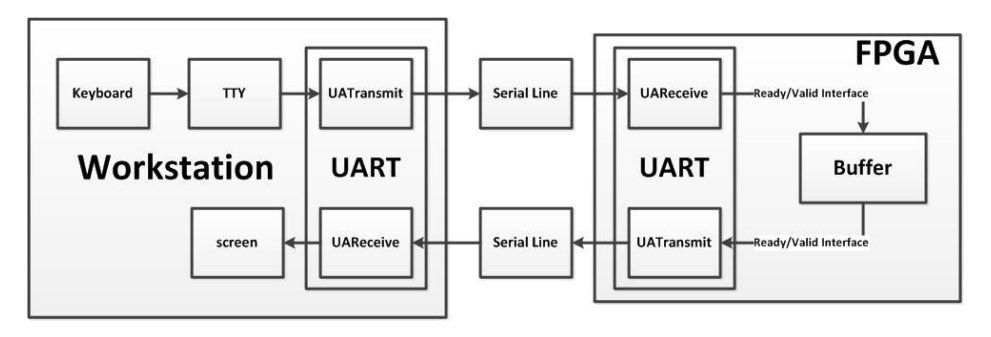
\includegraphics[width=6in]{figs/high_level_diagram.png}}
  \caption{High Level Diagram}
\end{figure}

In this lab, we'd like to ask you to implement both the \verb|uart_transmitter| and \verb|uart_receiver|.
In the process of testing your UART Receiver/Transmitter, if you see some weird garbage symbols then the data is getting corrupted and something is likely wrong.
If you see this happening very infrequently, don't just hope that it won't happen while the TA is doing the checkoff; take the time now to figure out what is wrong.
UART bugs are a common source of headaches for groups during the first project checkpoint.
We will provide many test modules to verify the robustness of your UART modules. You will be able to test your UART modules in action with a display monitor, keyboard, or a serial terminal.

\subsection{PMOD USB-UART}
The PYNQ-Z1 does not have an RS-232 serial interface connected to the FPGA fabric.
So we'll be using the \href{https://store.digilentinc.com/pmod-usbuart-usb-to-uart-interface/}{Pmod USB-UART} extension module to add a UART interface to the Pynq.
Connect the PMOD module to the \textbf{top} row of the PMOD A port on the Pynq, and connect a USB cable from the USB-UART PMOD to your computer.

\textbf{Note:} Make sure that the power selection jumper on the Pmod USBUART is set to LCL3V3

\subsection{Framing}
On the \verb|PYNQ-Z1| board, the physical signaling aspects (such as voltage level) of the serial connection will be taken care of by off-FPGA devices.
From the FPGA's perspective, there are two signals, \verb|FPGA_SERIAL_RX| and \verb|FPGA_SERIAL_TX|, which correspond to the receive-side and transmit-side pins of the serial port.
The FPGA's job is to correctly frame characters going back and forth across the serial connection.
Figure 1 below shows a single character frame being transmitted.

\begin{figure}[H]
  \centerline{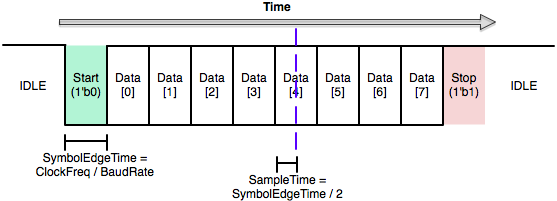
\includegraphics[width=6in]{figs/uart_frame.png}}
  \caption{UART Frame Structure}
\end{figure}

In the idle state the serial line is held high.
When the TX side is ready to send a character, it pulls the line low.
This is called the start bit.
Because UART is an asynchronous protocol, all timing within the frame is relative to when the start bit is first sent (or detected, on the receive side).

The frame is divided up in to 10 uniformly sized bits: the start bit, 8 data bits, and then the stop bit.
The width of a bit in cycles of the system clock is given by the system clock frequency divided by the baudrate.
The baudrate is the number of bits sent per second; in this lab the baudrate will be 115200.
Notice that both sides must agree on a baudrate for this scheme to be feasible.

\subsection{UART Receiver}

The receive side of the serial device is essentially just a shift register to shift bits from the serial line.
However, care must be taken into determining when to shift bits in.
If we attempt to sample the serial signal directly on the edge between two symbols, we are likely to sample on the wrong side of the edge and get the wrong value for that bit.
One solution is to wait halfway into a cycle (until \verb|SampleTime| on the diagram) before reading a bit in to the shift register.

One other subtlety of the receive side is correctly implementing the ready/valid interface.
Once we have received a full character over the serial port, we want to hold the valid signal high until the ready signal goes high, after which the valid signal will be driven low until we receive another character.

\textbf{Your task} is to complete the implementation of UART Receiver in the file \verb|lab6/src/uart_receiver.v|.

\subsubsection{Testing}

Use the following command to build your project with the UART Receiver module.

\begin{minted}{bash}
# This command builds a Vivado project named z1top_uart_rx_proj
# to interface with an IP.
make build-project proj=z1top_uart_rx
\end{minted}

This command loads all the necessary source files and constraint files to build your project. You can take a look at the file \verb|lab6/scripts/z1top_uart_rx.tcl| to see all the files required for this project. It also does some syntax checking to catch obvious bugs in your source file. You should pay attention to what prints out to the screen, and try to fix all the suspicious "WARNING" and "CRITICAL\_WARNING" messages before moving on. It might be helpful to run this command frequently after you make changes to your source files.

You can simulate your design with the provided testbench \verb|lab6/sim/uart_receiver_tb.v| by using the command

\begin{minted}{bash}
make sim proj=z1top_uart_rx tb=uart_receiver_tb
\end{minted}

The simulation will tell you if your design passes the testbench. To see the wavefor, you can open the Vivado project.

Once you are done with simulation, proceed to generate bitstream.

\begin{minted}{bash}
make write-bitstream proj=z1top_uart_rx
\end{minted}

This command launches Synthesis step, followed by Implementation step to generate a bitstream for your project. The bitstream is copied to \verb|lab6/bitstream_files|. Let's load the bitstream to configurate the FPGA with the following command.

\begin{minted}{bash}
make program-file bs=bitstream_files/z1top_uart_rx.bit
\end{minted}

You can take a look at the file \verb|lab6/src/z1top_uart_rx.v| to see what the top-level module does. Similar to the previous lab, it interfaces with a display controller for streaming image stored locally in the Block RAMs. However, the module has been extended to overwrite the existing image with a new one from the serial input (\verb|FPGA_SERIAL_RX|). Your UART Receiver will receiver a serial input from the host, and enqueue the pixel data to the module \verb|pixel_stream.v|. We will run a Python script to provide a new image data to the PYNQ via the serial interface.

\begin{minted}{bash}
python3 stream_img_from_serial.py
\end{minted}

If your module works correctly, when you hook a monitor to your PYNQ through an HDMI cable and turn on \verb|SWITCHES[1]|, you will see that the content of the current displayed image is being overwritten with a new image progressively from top to bottom.

Alternatively, if you don't have a monitor around, you can test your UART Receiver with a serial terminal on your workstation.

As an example, on your workstation, run:

\begin{minted}{bash}
screen $SERIALTTY 115200
\end{minted}

This tells \verb|screen|, a serial terminal, to open up the serial device with a baud rate of 115200 (you might have to run this with \verb|sudo| on your laptop). If \verb|$SERIALTTY| is not defined on your laptop, look for the name of the device file that the Serial Device is attached to, e.g. \verb|/dev/ttyUSB0| using \texttt{dmesg}. See the Appendix for more information.

When you type a character into the terminal, it is sent to the FPGA over the \verb|FPGA_SERIAL_RX| line, encoded in ASCII. Because we don't have a UART Transmitter yet, we won't be able to see the character echoed back to the screen for now! Try pressing a few keys and see if the LEDS show correct bit sequence of the ASCII code of the key you pressed. Note that \verb|SWITCHES[0] == 0| displays the four lower bits, and \verb|SWICHES[0] == 1| displays the four upper bits. Read the code to understand how the LEDS status is shown according to serial input. This is a low-stress test for UART Receiver module, since key pressing won't be as fast as a computer program.

To close \verb|screen|, type \verb|Ctrl-a| then \verb|Shift-k| and answer \verb|y| to the confirmation prompt.
If you don't close screen properly, other students won't be able to access the serial port on your workstation.

If you try opening \verb|screen| and it terminates after a few seconds with an error saying ``Sorry, can't find a PTY'' or ``Device is busy'', execute the command \verb|killscreen| which will kill all open screen sessions that other students may have left open.
Then run \verb|screen| again.

Use \verb|screen -r| to re-attach to a non-terminated screen session. You can also reboot the computer to clear all active \verb|screen| sessions.

\subsubsection{Debugging with Vivado Integrated Logic Analyzer (ILA)}

At some point, if you feel frustrated that you have tried all possible ways to debug your UART Receiver but it still does not work, you might likely want to use Vivado ILA to do in-system debugging. That means you will be able to load your bitstream, run your FPGA, interact with the board via external sources (buttons, keys pressed, etc.), and observe the waveform updated in real time! This could help you to catch bug that Simulation does not discover, since now you actually run your design on the FPGA. This is also really useful in situations where your FPGA has to interface with an external signal (such as \verb|FPGA_SERIAL_RX|), and you are uncertain if its behavior meets your assumption. This section aims to give you a short walkthrough to how to use Vivado ILA to debug your UART Receiver module. To learn more about Vivado ILA, you should take a look at its documentation \href{https://www.xilinx.com/support/documentation/sw_manuals/xilinx2019_2/ug908-vivado-programming-debugging.pdf}{Vivado Programming and Debugging}.

There are some signals in \verb|lab6/src/uart_receiver.v| and \verb|lab6/src/z1top_uart_rx.v| annotated with \verb|(* mark_debug = "true" *)|. This tells Vivado to not trim these signals during optimization, and that they will be monitored/probed during debugging session. Open your Vivado project in GUI mode (make sure your project has been implemented). In the \emph{Flow Navigator} panel, under \emph{Synthesis}, click \emph{Set Up Debug}.

\begin{center}
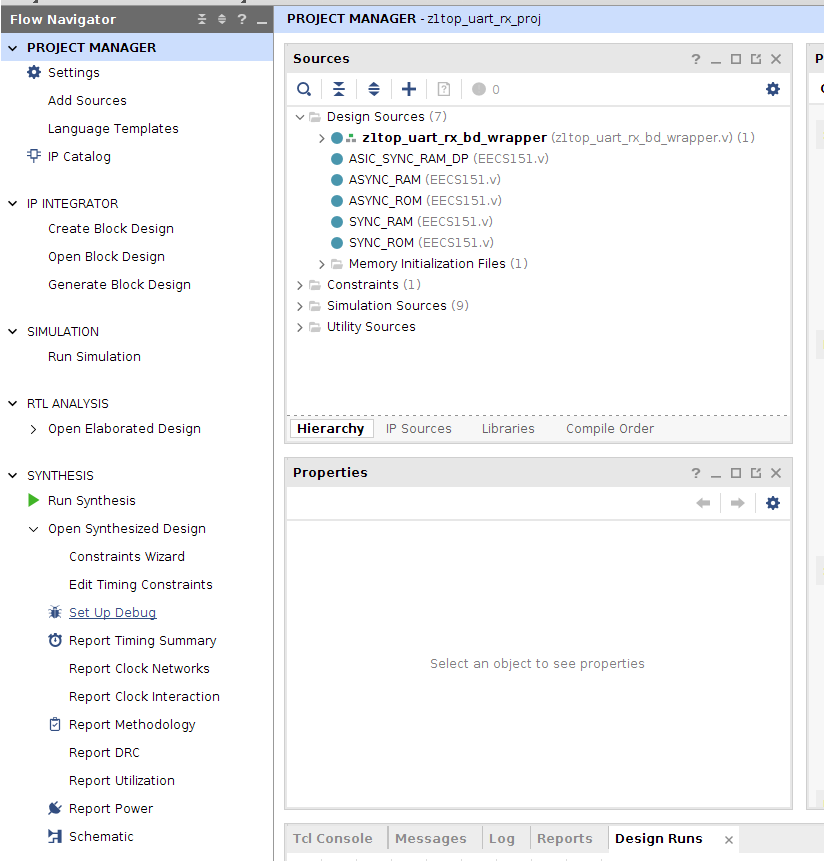
\includegraphics[width=0.4\textwidth]{figs/vivado-ila-1.png}
\end{center}

A wizard pops up to help you setup your debugging session. Click \emph{Next}. The list of signals marked with debug attributes are shown. You can also add other signals in this wizard. Notice the clock domain for each signal: this clock is used to sample debug data for the signal. Click \emph{Next}.

\begin{center}
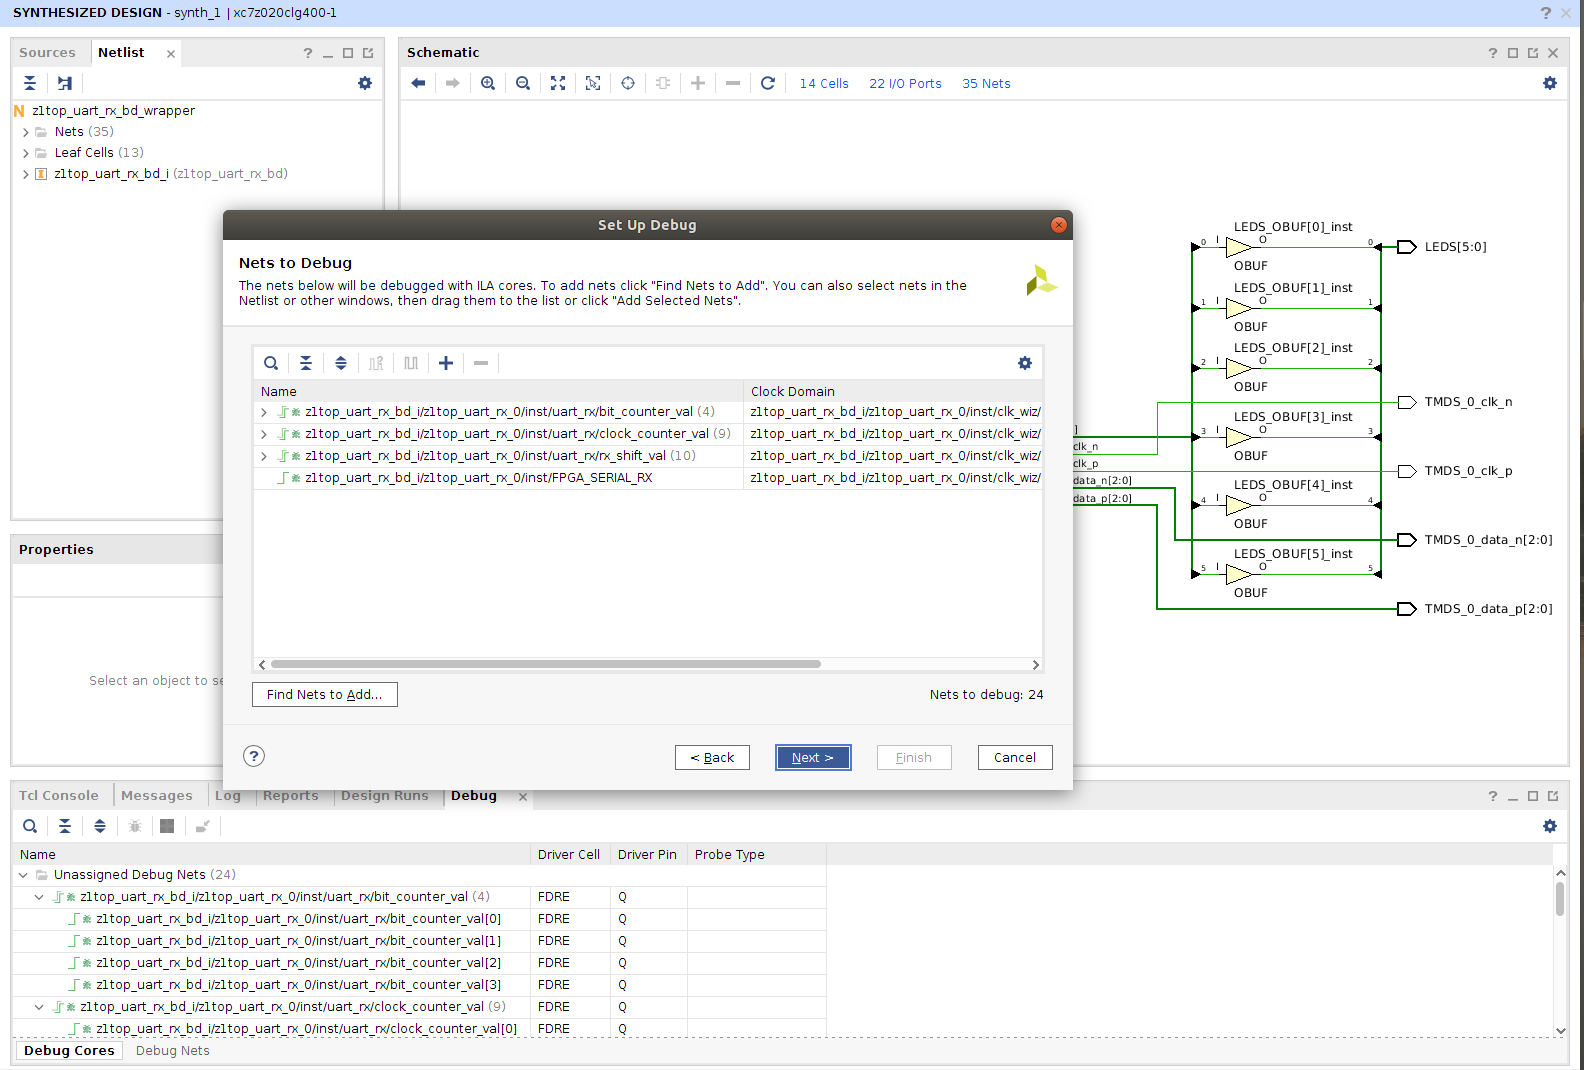
\includegraphics[width=0.7\textwidth]{figs/vivado-ila-2.png}
\end{center}

In this wizard, we will set the depth of the captured data (number of debug/captured data items) for our debugged signals. The bigger the depth value, the more debug data (or the longer the time) can be captured. However, since Vivado uses Block RAMs to store the captured data, your implementation might run out of on-chip memory storage if you set the depth too big. The debug cores actually consume resources; they are not free, so you should always be mindful of the current resource utilization of your design. In addition, make sure \emph{Capture control} and \emph{Advanced trigger} are checked. Hit \emph{Next}.

\begin{center}
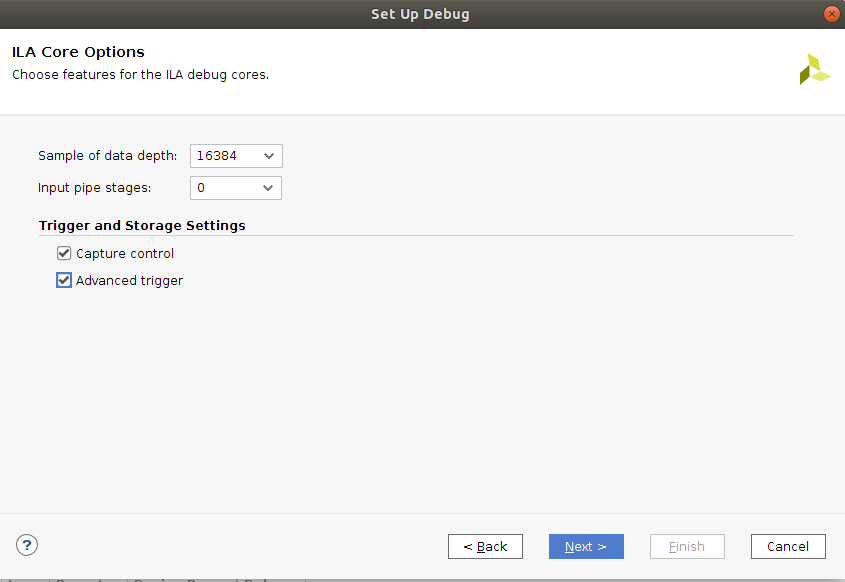
\includegraphics[width=0.7\textwidth]{figs/vivado-ila-3.png}
\end{center}

The following wizard asks where we should save the debug constraints. Select \emph{Create a new file} as in the following picture to avoid overwriting the existing constraint file. Click \emph{OK} to finish the debug setup. Now, we generate a new bitstream with the debug ILA cores: \emph{Generate Bitstream}.

After bitstream generation, we connect and program the FPGA as usual. This time, you will see that, in addition to the bitstream file, we also load the debug probes file.

\begin{center}
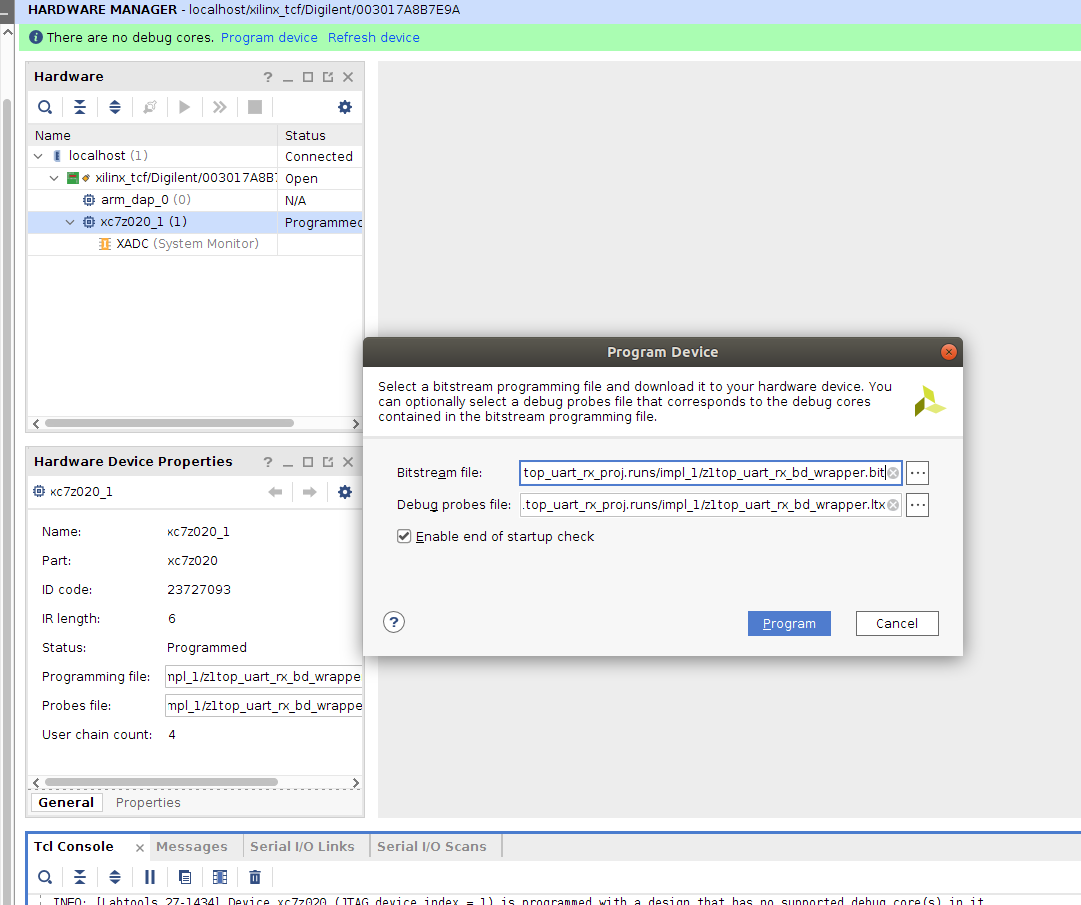
\includegraphics[width=0.7\textwidth]{figs/vivado-ila-5.png}
\end{center}

The waveform pane will show up after we program the FPGA with the probes file. This waveform window looks like the Simulation waveform window, but the cool thing is that we can setup trigger event to ignite the transitions of the signals we concern with. To do so, in the \emph{Trigger Setup - hw\_ila\_1} pane, click the plus button to add probes.

\begin{center}
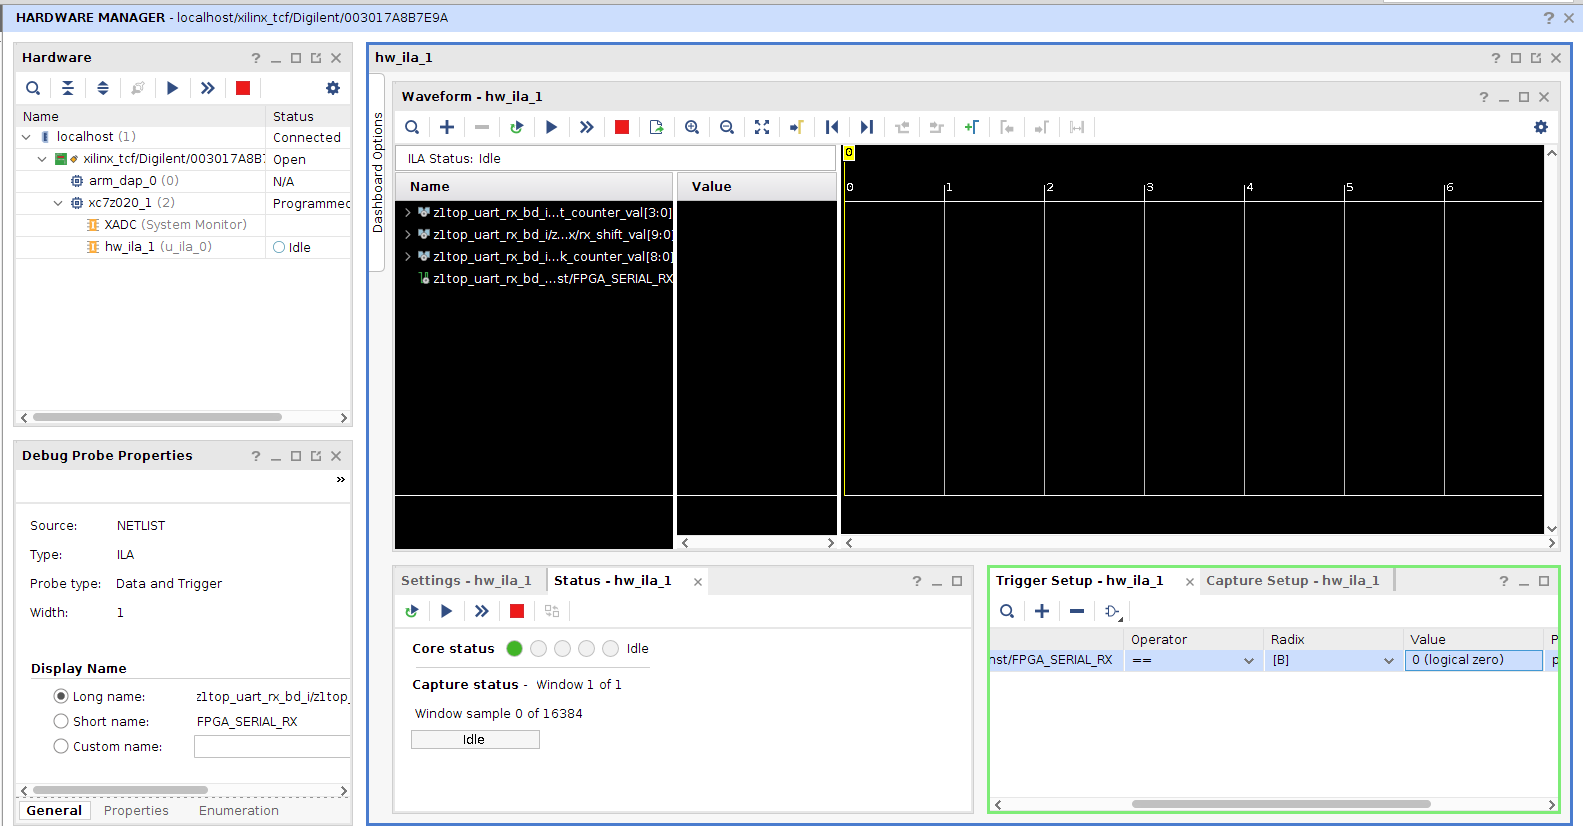
\includegraphics[width=0.7\textwidth]{figs/vivado-ila-7.png}
\end{center}

Select the signal \verb|FPGA_SERIAL_RX| from the popped-up window. Now, we will set the trigger condition. Also in the \emph{Trigger Setup - hw\_ila\_1} pane, select \emph{0 (logical zero} for the \emph{Value} column. The remaining columns can be kept unchanged. Essentially, we are comparing \verb|FPGA_SERIAL_RX| to 0: if the comparison is true, this will trigger the ILA cores. This makes sense, since the serial input is LOW when it wants to start a transaction; we want to begin capturing events at that moment.

\begin{center}
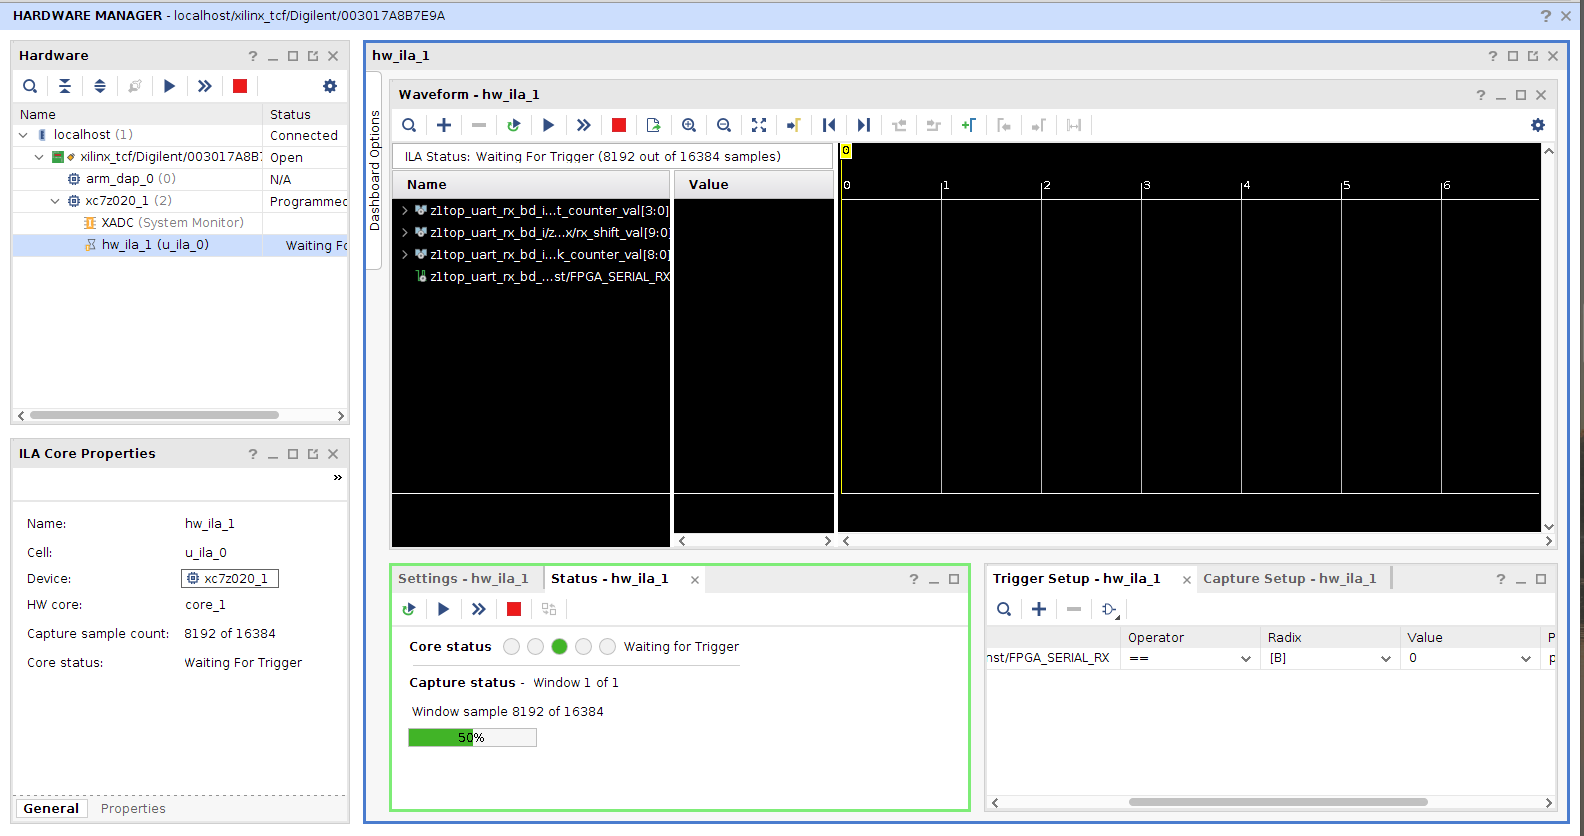
\includegraphics[width=0.7\textwidth]{figs/vivado-ila-8.png}
\end{center}

Now, in the \emph{Status - hw\_ila\_1} pane, click the play button ("Run trigger for this ILA core"). It will runs until waiting for trigger (50 \%). To complete the core execution, we will provide a \textbf{real} trigger from the serial terminal. Run

\begin{minted}{bash}
screen $SERIALTTY 115200
\end{minted}

on a separate terminal, and then press a key. This will send serial input to the PYNQ, and trigger the ILA core. Now you will see the waveform updated! The following picture shows one example which 'a' is pressed. You can see that \verb|rx_shift_val| is sampled in the middle of the symbol edge time, and one symbol edge time is roughly 345 cycles (note that we are using a clock of 40 MHz to drive the modules in this design). This is all happening when your PYNQ board is actually running.

\begin{center}
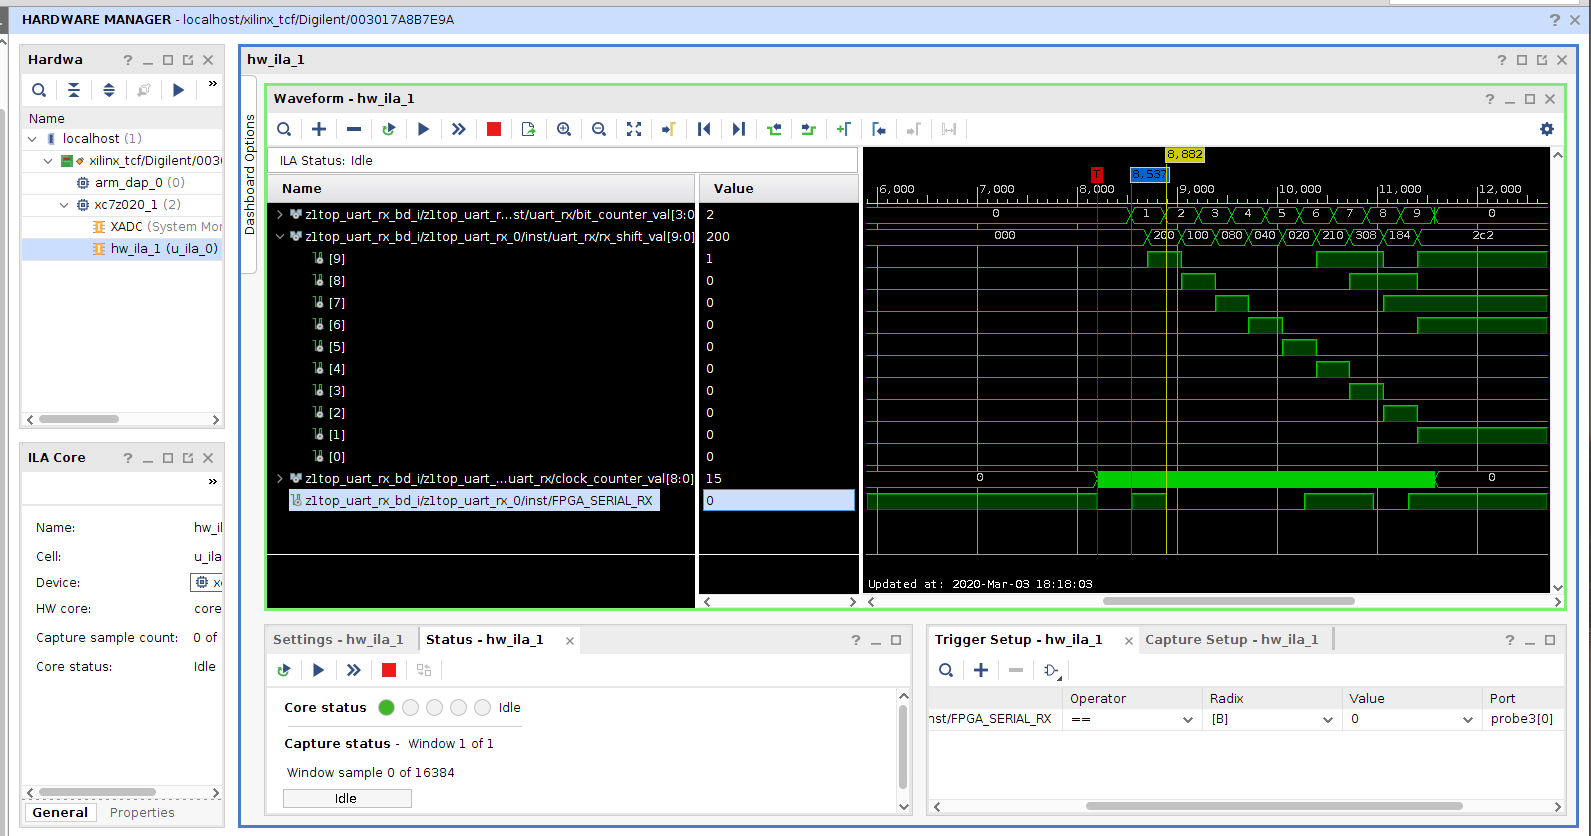
\includegraphics[width=0.7\textwidth]{figs/vivado-ila-9.png}
\end{center}

You can write a Python script to send multiple characters in a row to see if your design handles it correctly. Make sure your hardware window is big enough to store more events. Hopefully this example demonstrates to you how to use ILA to get meaningful messages from the system to debug your design.

\subsection{UART Transmitter}

Once we have a character that we want to send out, transmitting it is simply a matter of shifting each bit of the character, plus the start and stop bits, out of a shift register on to the serial line.

Remember, the serial baudrate is much slower than the system clock, so we must wait $SymbolEdgeTime = \frac{ClockFreq}{BaudRate}$ cycles between changing the character we're putting on the serial line.
After we have shifted all 10 bits out of the shift register, we are done unless we have to send another frame immediately after.

\textbf{Your task} is to complete the implementation of UART Transmitter in the file \verb|lab6/src/uart_transmitter.v|.

\subsubsection{Testing}

Similar to the previous exercise, you will need to use the following commands to build, implement, and test your project with the UART Transmitter module.

\begin{minted}{bash}

# Build Vivado project z1top_uart_tx_proj
make build-project proj=z1top_uart_tx

# Simulate with sim/uart_transmitter_tb.v
make sim proj=z1top_uart_tx tb=uart_transmitter_tb

# Generate bitstream
make write-bitstream proj=z1top_uart_tx

# Program the FPGA
make program-fpga bs=bitstream_files/z1top_uart_tx.bit
\end{minted}

If you are more comfortable with the GUI mode, you can open the Vivado project right after the \texttt{make build-project} command.

The \verb|z1top_uart_tx| module stores a text data locally in the block RAMs. The role of the UART Transmitter is to dequeue that data and send it to your workstation over the serial interface. You should be able to see the text on your serial terminal. Run

\begin{minted}{bash}
screen $SERIALTTY 115200
\end{minted}

After the FPGA is programmed, turn on \verb|SWITCHES[1]|. The text will appear on the serial terminal. You can also use the \verb|BUTTONS| and \verb|SWITCHES[0]| to provide input to the UART Transmitter. Read the code \verb|lab6/src/z1top_uart_tx.v| to see what should be expected.

\subsection{UART Echo -- Putting It All Together}

In this section, we will put both the UART Receiver and Transmitter together, and attempt to communicate with a serial terminal on your workstation. Use the following commands to build and implement your project.

\begin{minted}{bash}

# Build Vivado project z1top_uart_echo_proj
make build-project proj=z1top_uart_echo

# There is no testbench provided for this module

# Generate bitstream
make write-bitstream proj=z1top_uart_echo

# Program the FPGA
make program-fpga bs=bitstream_files/z1top_uart_echo.bit
\end{minted}

Now, open \verb|screen| as similar to previous sections. Try hitting your keyboard really hard and fast and see if you can get all the characters echoed back. Let's try an even harder test. We will run a Python script to read a text file on your local workstation, send the file to the PYNQ via the serial line, and observe the content of the file on a serial terminal.

\begin{minted}{bash}
# The command line argument is a text file to be sent over the serial line.
# Here is one example:
python3 scripts/echo.py src/z1top_uart_echo.v
\end{minted}

After the script prompts for user input, open \verb|screen| as usual in a separate terminal before hitting \texttt{Enter}. If everything goes well, you should see the text content shown in the serial terminal. Good work! Your UART Transmitter and Receiver are now thoroughly tested.

\section{Drawing Triangle}

This section intends to make you aware of timing closure problem in FPGA design. Timing closure is a process of optimizing your circuit to meet the target frequency. So far, we have been dealing with small circuit designs that utilize a few LUTs or FFs. The tool does not have any challenge in placement and routing your circuits to meet the timing (typically 125 MHz). In this section, we will work with a moderate-size circuit that involves lots of arithmetic operations, such as addition, subtraction, and multiplication of 32-bit nets. We will optimize the circuit to satisfy a target clock frequency. To do so, you should be aware of the critical path in your design. The critical path is the path between two registers (or flip-flops) that has the longest delay. One simple, yet powerful technique of improving the timing of a digital circuit is pipelining: we essentially place some registers on the critical path to break it into shorter paths. However, this will change the functionality of your design since now the path requires two cycles to complete instead of one. In addition, you must make sure that other signals involved with that path (e.g., using the output of the path, or providing input to the path) are also properly registered to ensure behavioral correctness of your pipelined circuit.


Let's look at a concrete example.

\begin{center}
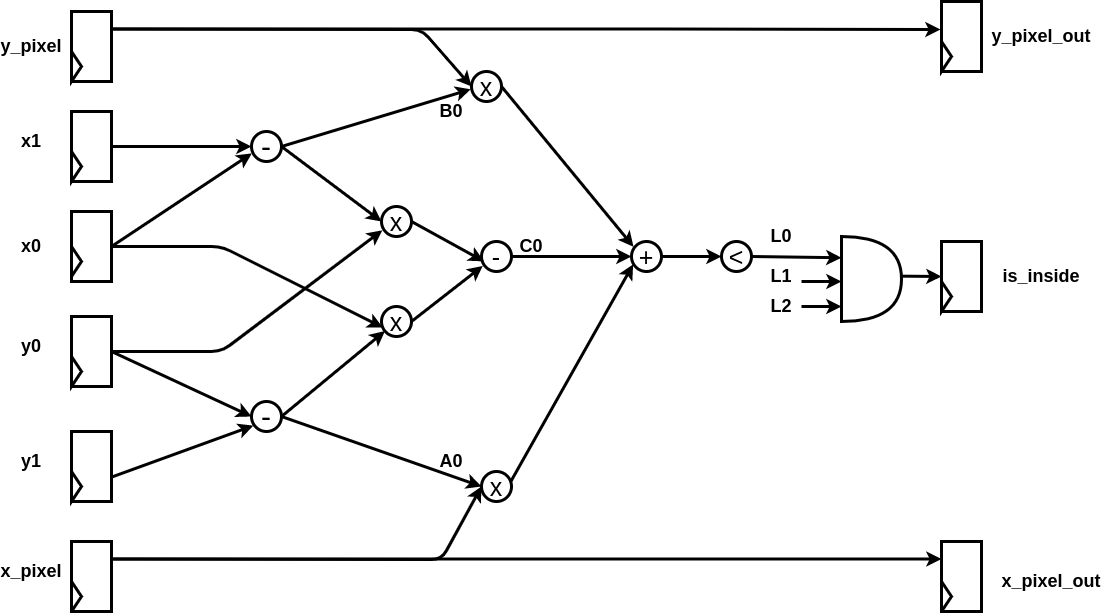
\includegraphics[width=0.6\textwidth]{figs/point_in_triangle.png}
\end{center}

This circuit (partially shown for brevity) does a point-in-triangle testing. Suppose we want to draw a triangle given the pixel coordinates of the three vertices. At every pixel of an image, we would like to test if the pixel is inside the triangle. One way of doing so is to test the relative position of the pixel to the lines formed by each pair of the three vertices. If the pixel is on the same side for all three lines, it is inside the triangle, and we assign the pixel with a color. You can read about it more from the \href{https://cs184.eecs.berkeley.edu/sp19/lecture/2/rasterization}{Computer Graphics course lecture}. However, you really don't need to know the detail of the math. We have provided you a working \verb|point_in_triangle| circuit design in the file \verb|lab6/src/point_in_triangle.v|. Your task is to figure out where to put pipeline stage(s) to meet the required clock frequency.

In addition, you need to modify the file \verb|lab6/src/draw_triangle.v| to implement proper video signals as in the \verb|display_controller.v|, but you should use \verb|x_pixel_out| and \verb|y_pixel_out| to drive the video signals instead. This module is similar to the \verb|display_controller.v|, except that now we stream a graphical object drawn by our circuit instead of a static image.

The file \verb|lab6/src/z1top_draw_triangle.v| is the top-level module that interfaces with Digilent video IP to draw a triangle to a monitor. It also instantiates the UART modules so that you can move the triangle using the keyboard of your workstation.
You only need to modify \verb|PIXEL_CLK_PERIOD| parameter to change the target pixel clock period of your system. For this exercise, we will configure video output with a resolution of 1024 $\times$ 768 @60Hz. That would require a pixel clock of 65 MHz. You are expected to pipeline the \verb|point_in_triangle| module to meet the target clock period of \textbf{16 ns}. To build and test your project, use the following commands.

\begin{minted}{bash}

# Build Vivado project z1top_draw_triangle_proj
make build-project proj=z1top_draw_triangle

# Simulate with sim/point_in_triangle_tb.v
make sim proj=z1top_draw_triangle tb=point_in_triangle_tb

# Generate bitstream
make write-bitstream proj=z1top_draw_triangle

# The timing report can be found at
# z1top_draw_triangle_proj/z1top_draw_triangle_proj.runs/\
# impl_1/z1top_draw_triangle_timing_summary.rpt

# Program the FPGA
make program-fpga bs=bitstream_files/z1top_draw_triangle.bit
\end{minted}

Every time you make change to the \verb|point_in_triangle| module, you should run a simulation to ensure that the functionality is still correct. A testbench has been provided for this purpose: \verb|lab6/sim/point_in_triangle_tb.v|. Once you pass the simulation, generate the bitstream and check the timing report to see if your design meets timing. A negative slack means a path in your design fails to meet the target clock period, and you should fix it. Look at the \textbf{VIOLATED} path(s) in the report, try to make sense of how that path corresponds to your Verilog code, and the delay at each primitives/sites on which the signal traverses that path, this should give you a hint of where to place your register(s) to cut the path. Since your design eventually boils down to FPGA primitives such as LUTs, FF, carry chains, or wires, sometimes it is difficult to tell exactly how the paths in the report are relevant to your Verilog source code. Nonetheless, you can make some educated guess of the delay of your path based on the dataflow graph of your circuit, as shown in the figure above. For instances, the delay on a path with a multiplier and a subtractor probably takes longer than a path with only an adder. Remember that FPGA is a spatial computing device, everything you write costs area and timing. Think carefully of which operators should you use. For example, if you want to scale a signal down, you probably need to think twice before using a divider; a right shift is much better in terms of hardware cost and is more FPGA-friendly. Depending on the quality of your FPGA board, a slightly negative-slack design can still work sometimes, but don't take it for granted. You should develop a practice of checking the timing report every time you finish implementation. If you believe you do everything right (up to Simulation), yet your design does not work on the board, check the timing.

%\newpage
\section{Lab Deliverables (due: 8PM, Mar 13th, 2020)}
\subsection{Lab Checkoff}
To checkoff for this lab, have these things ready to show the TA:
\begin{enumerate}
  \item Demonstrate that all modules \verb|z1top_uart_rx|, \verb|z1top_uart_tx|, and \verb|z1top_uart_echo| work properly. For all of your modules, you are expected to implement the state elements using REGISTER* modules from \verb|lib/EECS151.v| instead of sequential always block or non-blocking assignment.
  \item Demonstrate that your \verb|z1top_draw_triangle| module meets a pixel clock period of 16 ns.

\end{enumerate}

\subsection{Lab Report}\label{sec:labreport}

No lab report.

\appendix
\section{Personal Laptop Instructions}

\subsubsection{Linux/OSX}
After plugging in the USB cable, run \verb|dmesg| and observe the output:
\begin{minted}{text}
[7444636.941491] ftdi_sio 1-2:1.0: FTDI USB Serial Device converter detected
[7444636.941621] usb 1-2: Detected FT232RL
[7444636.942062] usb 1-2: FTDI USB Serial Device converter now attached to ttyUSB0
\end{minted}

Then connect using \verb|sudo screen /dev/ttyUSB0 115200|

\subsubsection{Windows}
After plugging in the USB cable, you may be prompted to install the FTDI drivers, so do that.
Follow the \href{https://xilinx-wiki.atlassian.net/wiki/spaces/A/pages/18842446/Setup+a+Serial+Console}{steps from here} to use PuTTY to connect to the UART.

%\newpage
\section*{Ackowlegement}
This lab is the result of the work of many EECS151/251 GSIs over the years including:
\begin{itemize}
\item Sp12: James Parker, Daiwei Li, Shaoyi Cheng
\item Sp13: Shaoyi Cheng, Vincent Lee
\item Fa14: Simon Scott, Ian Juch
\item Fa15: James Martin
\item Fa16: Vighnesh Iyer
\item Fa17: George Alexandrov, Vighnesh Iyer, Nathan Narevsky
\item Sp18: Arya Reais-Parsi, Taehwan Kim
\item Fa18: Ali Moin, George Alexandrov, Andy Zhou
\item Sp19: Christopher Yarp, Arya Reais-Parsi
\item Fa19: Cem Yalcin, Rebekah Zhao, Ryan Kaveh, Vighnesh Iyer
\end{itemize}

\end{document}
